\documentclass[tikz,border=3pt]{standalone}
\usepackage[utf8]{inputenc}
\usepackage[T1]{fontenc}
\usepackage{libertinus}
\usepackage{amsmath,amssymb}
\usetikzlibrary{arrows.meta,calc,patterns,decorations.pathmorphing,decorations.markings,decorations.pathreplacing,bending}
\definecolor{UGblue}{RGB}{0,51,102}
\newcommand{\dbar}{\mathchar'26\mkern-12mu d}
\tikzset{
  >=Stealth,
  every node/.style={font=\small},
  caja/.style={draw,line width=0.9pt},
  pared/.style={draw,line width=1.6pt},
  ejes/.style={->,line width=0.8pt},
  adia/.style={draw,pattern=north east lines,pattern color=black!70,line width=0.5pt},
  gas/.style={fill=UGblue!8},
  punto/.style={fill,circle,inner sep=1.3pt},
  onda/.style={decorate,decoration={snake,amplitude=1.1pt,segment length=5pt,post length=3pt,pre length=0pt}},
}
\begin{document}
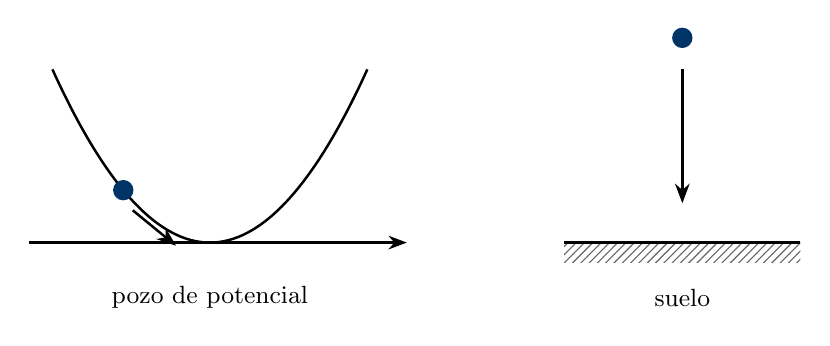
\begin{tikzpicture}
  % pozo
  \draw[line width=0.9pt,domain=0:4,samples=60,smooth,variable=\x] plot ({\x},{0.55*(\x-2)*(\x-2)});
  \draw[ejes] (-0.3,0) -- (4.5,0);
  \node[circle,fill=UGblue,inner sep=2.6pt] (p) at (0.9,0.55*1.21) {};
  \draw[->,line width=0.9pt] (0.9,0.67) ++(0.12,-0.26) -- ++(0.55,-0.45);
  \node at (2,-0.7) {pozo de potencial};
  % caída
  \begin{scope}[xshift=6.5cm]
    \path[pattern=north east lines,pattern color=black!60] (0,-0.25) rectangle (3,0);
    \draw[line width=0.9pt] (0,0) -- (3,0);
    \node[circle,fill=UGblue,inner sep=2.6pt] at (1.5,2.6) {};
    \draw[->,line width=0.9pt] (1.5,2.2) -- (1.5,0.5);
    \node at (1.5,-0.7) {suelo};
  \end{scope}
\end{tikzpicture}
\end{document}
